\section{GHio-Ca}
In this section we will provide some salient features implemented by our
application, mainly regarding the architectural and implementation choices that
we made developing the code.

\subsection{Architecture}
GHio-Ca is principally composed of two layers: (i) the layer that have to manage
network connectivity, uploading photos to the server and making requests to
different services in order to make the image recognition or the translation of
certain pieces of text, and (ii) the camera layer, that manages the photo
capturing process and saving.

These two layers are maintained as loose coupled as possible in order to make
easy to change services used without making important changes to the overall
application or changing the process of photo taking, without modify the
networking layer.

%TODO
%	-add a UML of the application architecture at really high level
%		   NETWORK
%
%		|-----------|           |---------------|
%		| LISTENERS |------>    |     PHOTO     |
%		| ASYNCTASK |<------    |               |
%		|-----------|           |---------------|

\subsection{Application description}
GHio-Ca (Giving Hashtags In Order To Classify Automatically) is an Android
application that gives to a user the possibility to make image recognition on
her pictures. This application embed some camera features in order to make
possible to take a photo and recognize it directly, but it also allows to pick
a picture from the saved ones and launch the classifying process on it.
GHio-Ca is specifically designed to recognize objects and text: the only
limitation is that the user has to choose it before starting the
recognition process from the hamburger menu placed in the main activity.
The overall application is mainly composed by four activities:
\begin{itemize}
  \item splash activity: this view is needed in order to gain from the user
    the necessary permissions (network access, camera access, access to
    the storage);
    \begin{figure}[h]
        \centering
        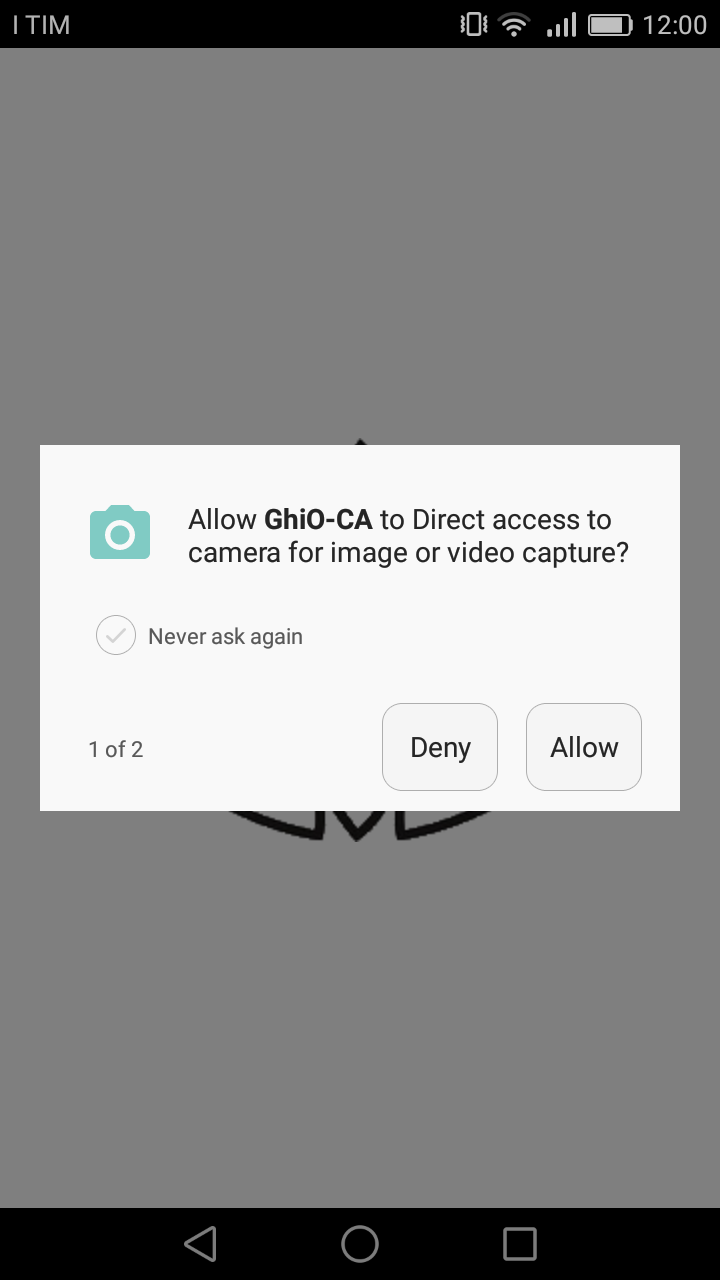
\includegraphics[width=0.18\textwidth]{../img/splash}
        \caption{Screen-shot of the splash activity, when authorization are 
                 required}
        \label{fig:splash}
    \end{figure}
  \item camera preview activity: this one displays the user a camera
    interface, with the possibility to take photos, turn off the flash, switch
    to frontal camera (if present) and to access to the gallery in order to
    pick a file instead of taking a picture. In the top left corner is present
    the hamburger menu: it allows user to choose the size of picture taken,
    it reminds the user to turn on the Wi-Fi sensor on every access and it
    allows to switch from the image recognition functionality to the
    character optical recognition feature and vice-versa;
    \begin{figure}[h]
        \centering
        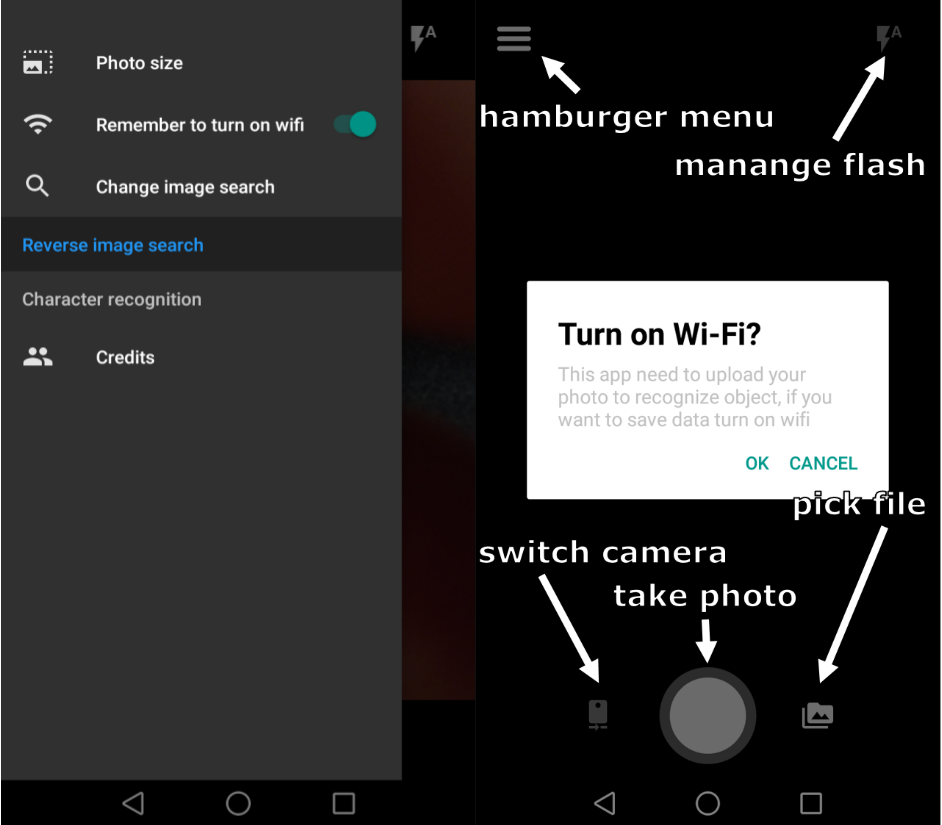
\includegraphics[width=0.30\textwidth]{../img/main_activity}
        \caption{Screen-shots of the main activity, with and without open 
                 hamburger menu}
        \label{fig:splash}
    \end{figure}
  \item results activities: these are two different activities depending on
    the type of image recognition chosen.
    \begin{itemize}
     \item If the ``reverse image search'' functionality is enabled then the
result activity will contain a photo thumbnail, a description and a list of
tags. Any tag can be deselected by the user if it doesn't fit the image.
    \begin{figure}[h]
        \centering
        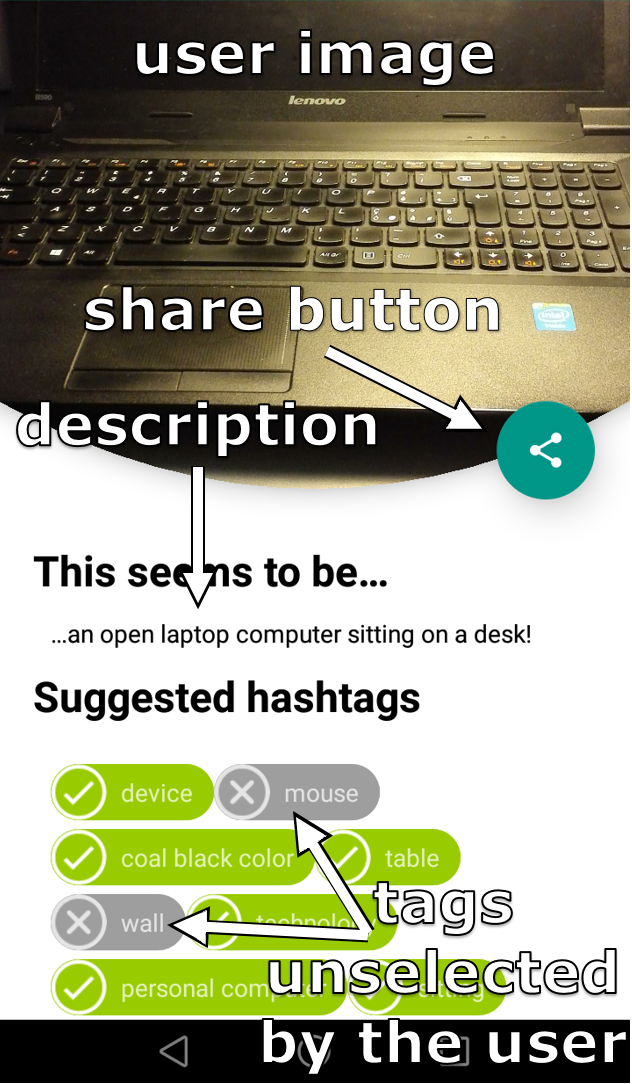
\includegraphics[width=0.18\textwidth]{../img/image_result_activity}
        \caption{Screen-shots of the result activity for image recognition}
        \label{fig:splash}
    \end{figure}
     \item With ``optical character recognition'' on, instead, the result
activity will display the photographed text and its OCR translation. The user
will be able to pick another translation from a drop down menu.
    \end{itemize}
\end{itemize}